\index{general}{Domain Decomposition}

%---------------------------
\subsubsection{Rationale}

Let us assume that we want ro run a simulation of the whole Earth mantle
with a constant resolution of $5\text{km}$. The volume of the mantle is
\[
V_{mantle}=\frac{4}{3}\pi (R_{out}^3-R_{in}^3) \simeq  10^{12}  km^3
\]
while the volume of an element is $V_{e} = 125 \text{km}^3$ (this is 
only an average since the tesselation of a hollow sphere with 
hexahedra yields elements which are not all similar \cite{thie18}).
Consequently, the number of cells needed to discretise the mantle
is 
\[
N_{el}=\frac{V_{mantle}}{V_{e}}\simeq 8\times 10^9
\]
We know that the matrix size is approx. 4 times the number of elements in 3D:
\[
N\simeq 25 \times 10^9
\]
Using between 9 and 125 particles per element (a very conservative number),
the total number of particles is then
\[
N_{particles}  \geq 10^{10}
\]
The unescapable conclusion is that high-resolution 3D 
calculations 
 have a very large memory footprint and require extremely long computational times.

The only way to overcome this problem is by resorting to 
using supercomputers with many processors and large memory capacities.

The idea behind parallel programming is to have each processor carry out 
only a subset of the total number of operations required. In order to reduce 
the memory footprint on each processor, only a subset of the computational
mesh is known by each: one speaks then of domain decomposition \cite{towi}.

An example of such a large parallel calculation of 3D convection with 
domain decomposition in a spherical shell can be found in \cite{krhb12}:

\begin{center}
a)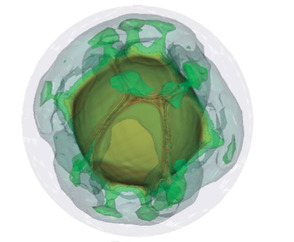
\includegraphics[width=7cm]{images/parallel/krhb2}
b)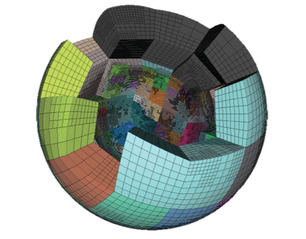
\includegraphics[width=7cm]{images/parallel/krhb1} \\
{\captionfont a)Isocontours of the temperature field; b) Partitioning of the domain onto 512 proc. 
The mesh counts 1,424,176 cells. The solution has approximately 54 million unknowns 
(39 million vel., 1.7 million press., and 13 million temp.)
}
\end{center}

%---------------------------
\subsubsection{Basic approaches}

In the past, many applications implemented the idea below on the left using 1D domain decomposition 
(also known as ``slab decomposition''). In the following left figure, 
a 3D domain is arbitrarily chosen to be decomposed in Y and X directions. 
It can be seen that in state (a), any computations in the X-Z planes can be done in local memories 
while data along a Y mesh-line is distributed. 

\begin{center}
a)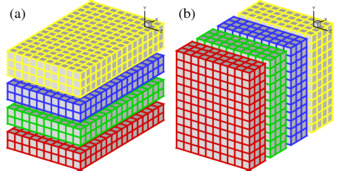
\includegraphics[width=5cm]{images/parallel/dd1}
\hspace{1cm}
b)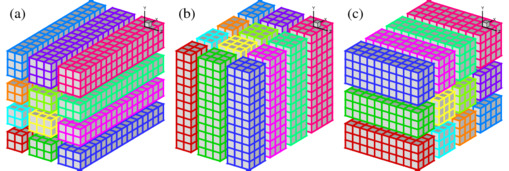
\includegraphics[width=7cm]{images/parallel/dd2}\\
{\captionfont Left: 1D domain decomposition example using 4 processors: 
(a) decomposed in Y direction; (b) decomposed in X direction.
Right: 2D domain decomposition example using a 4x3 processor grid.}
\end{center}

A $1D$ decomposition, while quite simple, has some limitations, especially for large-scale simulations. 
Given a cubic mesh of size $N^3$ , one obvious constraint is that the maximum number of processors 
Nproc that can be used in a 1D decomposition is $N$ as each slab has to contain at least one plane
\footnote{This domain decomposition approach is the one carried out in the FANTOM code \cite{thie11}
and this limitation was often encountered when using grids such as 160x160x23, thereby limiting the number 
of processors to about 100 processors.}
For a cubic mesh with $1000^3=10^9$ points, the constraint is $Nproc \leq 1000$. 
This is a serious limitation as most supercomputers today have more than 
10,000 cores and some have more than 100,000. 
Large applications are also likely to hit the memory limit when each processor handles too much workload. 



%---------------------------
\subsubsection{Load balancing}

\index{general}{Load Balancing}
\index{general}{Space Filling Curve}

In computing, load balancing distributes workloads across multiple computing resources, such as computers, a computer cluster, network links, central processing units or disk drives. Load balancing aims to optimize resource use, maximize throughput, minimize response time, and avoid overload of any single resource. 

More concretely, the use of many processors in the case where the mesh is unstructured and highly irregular 
raises the question of how the partitioning is done so that each processor gets a similar workload, thereby 
minimising latency and optimising cpu time.

This is a difficult problem which is often addressed by means of graph partitioners, and which is made 
more complicated by the use of AMR. 

A typical strategy goes as follows. One can prove that {\bf space filling curves}
can be generated for any regular subdivision of a square (see dashed line in the following
figure).

\begin{center}
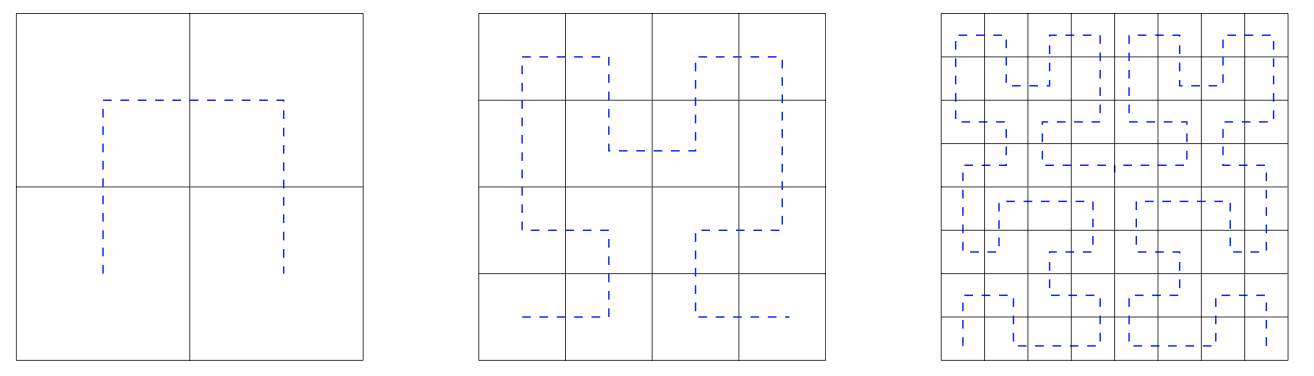
\includegraphics[width=8cm]{images/parallel/sfc1}
\end{center}

It now the refined grid is the one shown on the following figure, one can use the curve to 'write'
all elements in a line and then cut this curve in Nproc chunks (in this case 4, hence four colours).

\begin{center}
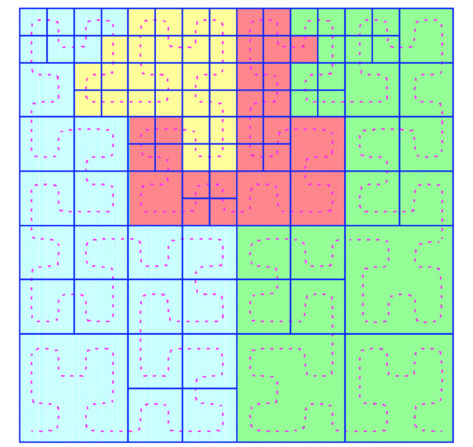
\includegraphics[width=5cm]{images/parallel/sfc2}
\end{center}

The mesh counts in total 100 elements and each domain counts 25 elements. 
This decomposition looks very appealing but another aspect must be taken in account:
communication.

Ideally, one wishes to carry out the domain decomposition in a simple-enough manner so that 
it does not require too much work, and also in such a way that the surface between between 
all the domain is minimised, since it is related to the amount of communication 
across processors.  

The following figures showcase examples of domain decomposition projected 
onto a complex 3D geometry.

\begin{center}
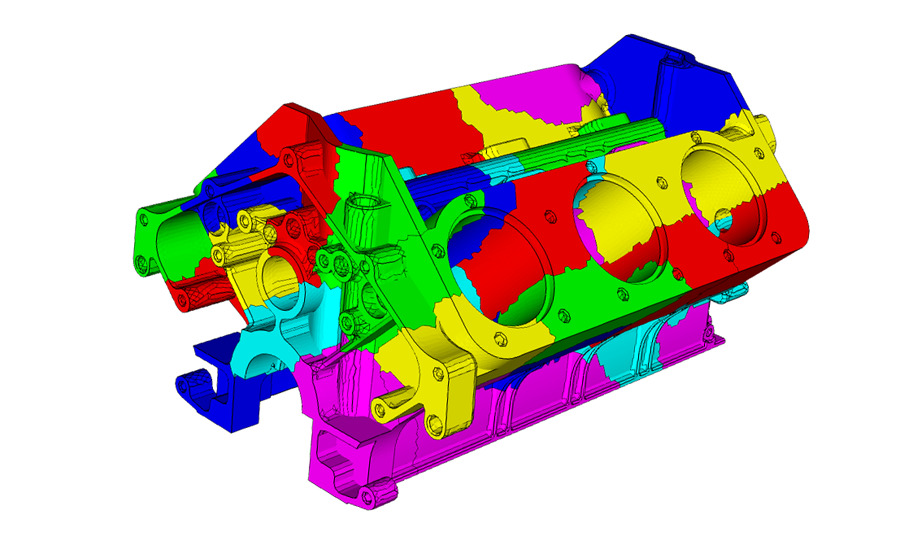
\includegraphics[width=8cm]{images/parallel/engine}
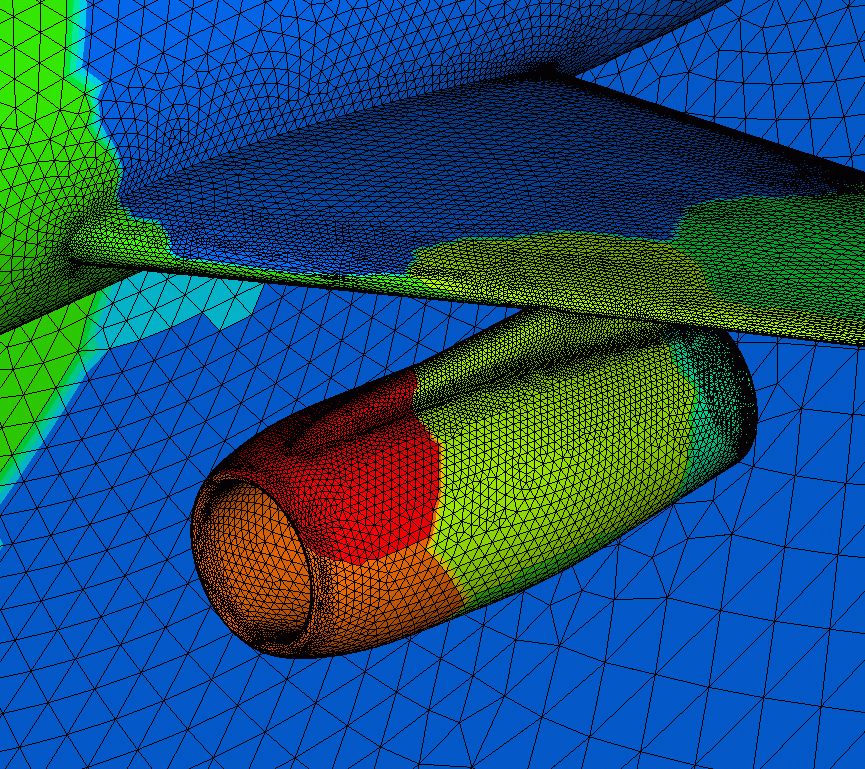
\includegraphics[width=5.5cm]{images/parallel/wing}\\
{\captionfont Right: Domain decomposition for parallel processing of a wing-body-nacelle-pylon configuration.
Each colour corresponds to a different processor.}
\end{center}







%----------------------------------------------
\subsubsection{Strong scaling vs weak scaling}

\begin{center}
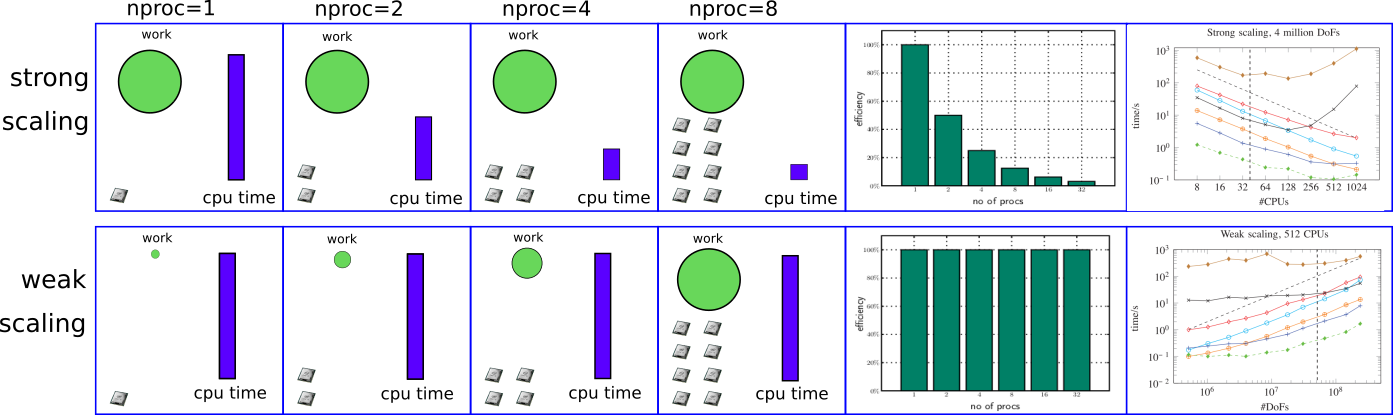
\includegraphics[width=16cm]{images/parallel/fig}
\end{center}


